% *********************************************************************
% © 2016–2025 Jeremy Sylvestre
%
% Permission is granted to copy, distribute and/or modify this document
% under the terms of the GNU Free Documentation License, Version 1.3 or
% any later version published by the Free Software Foundation; with no
% Invariant Sections, no Front-Cover Texts, and no Back-Cover Texts. A
% copy of the license is included in the appendix entitled “GNU Free
% Documentation License” that appears in the output document of this
% PreTeXt source code. All trademarks™ are the registered® marks of
% their respective owners.
%
% *********************************************************************
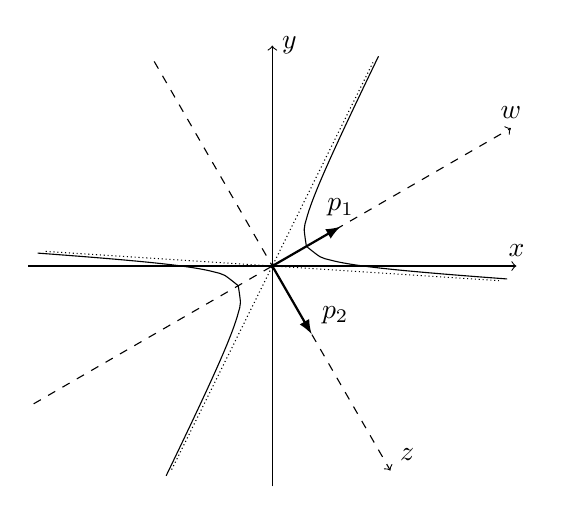
\begin{tikzpicture}[
	point/.style={circle,draw,very thin,fill,inner sep=0pt,minimum size=4pt},
	vector/.style={-latex},
]

	\draw[->] (-3.1,0) to (3.1,0) node[above] {$x$};
	\draw[->] (0,-2.8) to (0,2.8) node[right] {$y$};

	\begin{scope}[rotate=-60]

		\draw[dashed,->] (0,-3.5) to (0,3.5) node[above] {$w$};
		\draw[dashed,->] (-3,0) to (3,0) node[above right] {$z$};

		\draw[domain=0.5:2.5,smooth,variable=\t] plot ({sqrt(4 * \t * \t - 1) / 3},\t);
		\draw[domain=0.5:2.5,smooth,variable=\t] plot ({sqrt(4 * \t * \t - 1) / 3},{-\t});
		\draw[domain=0.5:2.5,smooth,variable=\t] plot ({-sqrt(4 * \t * \t - 1) / 3},\t);
		\draw[domain=0.5:2.5,smooth,variable=\t] plot ({-sqrt(4 * \t * \t - 1) / 3},{-\t});

		\draw[densely dotted] (-1.6,-2.4) -- (1.6,2.4);
		\draw[densely dotted] (1.6,-2.4) -- (-1.6,2.4);

	\end{scope}

	\draw[vector,thick] (0,0) to (0.866,0.5) node[above] {$\uvec{p}_1$};
	\draw[vector,thick] (0,0) to (0.5,-0.866) node[above right] {$\uvec{p}_2$};

\end{tikzpicture}
